\documentclass[11pt]{article}
\usepackage[a4paper,margin=22mm]{geometry}
\usepackage{amsmath,amssymb,booktabs,longtable,array,graphicx,hyperref}
\DeclareUnicodeCharacter{2218}{\ensuremath{\circ}}
\title{A054 v0.6.0: E013 Provider-Convergent State-Selection Falsifier}
\author{Omar Iskandarani}
\date{2026}
\begin{document}\maketitle
% SST-REPORT-SECTION:IDENTIFICATION
\section{Identification}
This v0.6.0 software migration preserves the parent scientific hypotheses and numerical thresholds. It does not execute state selection, Hessian, ringdown, native parity or reveal. The public migration protocol is frozen separately from any future complete blind campaign.

Catalog ID A054; release v0.6.0; SST Falsifier Framework v1.0.10, registered profile \texttt{multilibrary\_gpu}; this execution uses only the bounded ADMISSION\_SMOKE lane. This is an E013 cross-falsifier member at stage 30.
% SST-REPORT-SECTION:QUESTION
\section{Question}
Can distinct current E011/PKLSA provider representatives of the same topology be mapped by one target-free variational selector to a common stationary and locally stable finite-core state?
% SST-REPORT-SECTION:HYPOTHESES
\section{Hypotheses}
The null states that provider dependence survives target-free state selection or that selected stationary states fail local stability. The alternative requires provider-convergent stationary and stable endpoints without topology/provider-specific retuning.
% SST-REPORT-SECTION:ASSUMPTIONS
\section{Assumptions}
E013 fixes the current carrier population. The selector is a variational existence/selection test, not a claim that inviscid Euler flow is dissipative. Physical stability is tested separately after stationarity. Legacy falsifier results are excluded as evidence.
% SST-REPORT-SECTION:SYMBOLS
\section{Symbols}
All hatted lengths, deformation coordinates and the comparison Hamiltonian are dimensionless under the registered reach normalization. No calibrated SI length, time, energy or physical dissipation is inferred.

$\widehat H_a$ is the reach-normalized regularized line-energy kernel, $q$ Bishop-frame deformation coordinates, $\sigma$ the normalized energy-gradient stationarity score, and $K_H$ the endpoint Hessian.
% SST-REPORT-SECTION:EQUATIONS
\section{Equations}
% AUTO-GENERATED. Do not edit; generated from frozen science_contract.json.
\subsection*{Machine-readable science contract}
\begin{description}
\item[Research question] On one E013-frozen population of current E011 provider anchors, can a fixed target-free variational state-selection procedure map distinct source representatives of the same topology to a common stationary and locally stable finite-core state, without using legacy falsifier results?
\item[Objective] Re-run state selection from source-native bytes for exactly the E013 carriers using one canonical constrained objective Uc(q)=H(N[R(X+deltaX(q))]) for gradient, Armijo line search, Hessian and ringdown; quantify stationarity, topology preservation, provider-endpoint convergence and local stability; numerical inability to demonstrate descent or Hessian-sign convergence is UNRESOLVED rather than a scientific FAIL; freeze only provider-converged stable endpoints as a future A057 handoff.
\item[$H_0$] H0: provider-distinct current PKLSA/SKLSA representatives do not converge under the preregistered selector to a reproducible stationary and stable topology-level state beyond numerical/source variation.
\item[$H_1$] H1: the same preregistered selector, without topology/provider-specific retuning, yields provider-convergent stationary and locally stable endpoints for a reproducible subset of topologies.
\end{description}
\subsubsection*{Registered equations}
\paragraph{E1: Regularized finite-core comparison Hamiltonian}
\begin{equation}
\widehat H_a=\sum_{i,j}\oint\!\oint \frac{d\widehat{\mathbf X}_i\cdot d\widehat{\mathbf X}_j}{\sqrt{\|\widehat{\mathbf X}_i-\widehat{\mathbf X}_j\|^2+\widehat a^2}}
\end{equation}
\noindent\textit{Dimensional check:} All lengths are reach-normalized; the kernel is dimensionless.\\
\paragraph{E2: Bishop-Fourier reduced deformation}
\begin{equation}
\delta\mathbf X(q)=\sum_\mu q_\mu\mathbf B_\mu,\qquad \mathbf B_\mu\perp\mathbf t
\end{equation}
\noindent\textit{Dimensional check:} In reach-normalized coordinates both q and B are dimensionless.\\
\paragraph{E3: Canonical constrained objective and stationarity score}
\begin{equation}
\mathcal P=\mathcal N\circ\mathcal R,\qquad U_c(q;X)=\widehat H_a\!\left(\mathcal P[X+\delta X(q)]\right),\qquad \sigma=\frac{\|\nabla_q U_c(0;X)\|_2}{\max(|U_c(0;X)|,\epsilon)}
\end{equation}
\noindent\textit{Dimensional check:} Projection and the reach-normalized Hamiltonian are dimensionless, so U\_c and sigma are dimensionless.\\
\paragraph{E4: Target-free Armijo/trust-region selector on the constrained objective}
\begin{equation}
d_n=-\frac{\nabla U_c}{\|\nabla U_c\|},\qquad \eta_{n,k}=\min(\Delta_n,\eta_0)\beta^k,\qquad U_c(\eta_{n,k}d_n)\le U_c(0)+c_1\eta_{n,k}\nabla U_c\!\cdot d_n
\end{equation}
\noindent\textit{Dimensional check:} q, trust radius and U\_c are dimensionless in the reach-normalized lane.\\
\paragraph{E5: Accepted-step integrity conditions}
\begin{equation}
\widehat H_{n+1}\le\widehat H_n,\quad d_{\min,n+1}\ge f_c d_{\min,0},\quad |\Delta Lk|\le\varepsilon_{Lk}
\end{equation}
\noindent\textit{Dimensional check:} Energy comparison is dimensionless; distance is compared as a ratio; linking is dimensionless.\\
\paragraph{E6: Cross-provider endpoint agreement}
\begin{equation}
CV_H(K)=\frac{s(H_K^*)}{|\overline H_K^*|},\qquad \Delta_R(K)=\frac{R_{\max}^*-R_{\min}^*}{|\overline R^*|}
\end{equation}
\noindent\textit{Dimensional check:} Coefficient of variation and relative spans are dimensionless.\\
\paragraph{E7: Constrained-objective Hessian with finite-difference sign convergence}
\begin{equation}
K_H^{(j)}=\nabla_q^2U_c(0;\epsilon/2^j),\quad j=0,1,2;\qquad \mathrm{promote\ sign}\iff s_0=s_1=s_2\ \land\ \frac{\|K_H^{(2)}-K_H^{(1)}\|_F}{\max(\|K_H^{(2)}\|_F,\epsilon)}\le\tau_H
\end{equation}
\noindent\textit{Dimensional check:} The reduced coordinates and U\_c are dimensionless, so all Hessian entries/eigenvalues are dimensionless.\\
\paragraph{E8: Nonlinear reduced ringdown on the same constrained objective}
\begin{equation}
\ddot z=-\partial_z U_c(z\,e_{\min}),\qquad e_{\min}=\operatorname*{argmin}_{\|e\|=1}e^TK_He
\end{equation}
\noindent\textit{Dimensional check:} Normalized time, z and U\_c make the reduced test dimensionless.\\
\paragraph{E9: State-selected handoff predicate}
\begin{equation}
Q_K=I[\mathrm{provider\ consensus}]I[\sigma\le\sigma_{\max}]I[K_H\succeq0]I[\mathrm{ringdown\ bounded}]
\end{equation}
\noindent\textit{Dimensional check:} Boolean predicate.\\
\subsubsection*{Registered code-to-mathematics steps}
\begin{enumerate}
\item \textbf{S1} [G0; equations E1]: Verify frozen protocol/implementation and exact E013/E011 source-byte binding.
\item \textbf{S2} [G1; equations E1]: Reload only E013-frozen carriers and recheck geometry hashes.
\item \textbf{S3} [G2; equations E1, E3, E4, E5]: Validate rigid-energy invariance, exact constrained-objective evaluation, Armijo monotonicity and topology-proxy mechanics.
\item \textbf{S4} [G3; equations E2, E3, E4, E5]: Run the fixed constrained-objective variational selector independently on every current carrier; classify failure to demonstrate numerical descent as UNRESOLVED\_NUMERICAL.
\item \textbf{S5} [G4; equations E3, E4]: Evaluate fixed-selector transfer on registered confirmation topologies.
\item \textbf{S6} [G5; equations E1]: Certify the common energy kernel against C++/OpenMP FP64.
\item \textbf{S7} [G6; equations E1]: Record optional GPU/DD32 framework screening without promotion.
\item \textbf{S8} [G7; equations E6]: Compare independently sourced endpoints topology-by-topology.
\item \textbf{S9} [G8; equations E7, E8]: Qualify stationary endpoints only after constrained-Hessian eps/2/4 convergence and then nonlinear ringdown on the same U\_c.
\item \textbf{S10} [G10; equations E6]: Test whether initially provider-sensitive energy kernels collapse after selection.
\item \textbf{S11} [G11; equations E5]: Audit clearance/linking topology proxies over all paths.
\item \textbf{S12} [G12; equations E9]: Freeze only provider-converged stable endpoints as a future A057 handoff.
\item \textbf{S13} [G22; equations E3, E6, E7, E9]: Assign the blind overall state-selection classification under diagnostic continuation.
\item \textbf{S14} [G9; equations E9]: Reserve framework reveal integrity gate; v0.6.0 contains no mass target reveal.
\end{enumerate}

% SST-REPORT-SECTION:ALGORITHM
\section{Algorithm}
The registered full algorithm reloads carriers and evaluates one constrained objective $U_c(q)=\widehat H_a(\mathcal N[\mathcal R(X+\delta X(q))])$. The same $U_c$ supplies finite-difference gradients, Armijo/trust-region acceptance, stationarity, endpoint Hessians, and nonlinear reduced ringdown. Accepted steps must preserve a nonlocal-clearance floor and pairwise linking within tolerance. Failure to demonstrate numerical descent is recorded as \texttt{UNRESOLVED\_NUMERICAL}, not as negative physical evidence.
% SST-REPORT-SECTION:SOURCES
\section{Sources}
E011-v0.3.0 is the static-seed/provider authority; E013-v0.1.1 freezes the common carrier population; E010-v0.3.1 only reloads the exact source-native geometry bytes. No old A054 output is a science input.
% SST-REPORT-SECTION:GATES
\section{Gates and diagnostic continuation}
Only G0 is a hard prerequisite. Scientific failures do not suppress later diagnostics. Soft dependency caveats prevent a numerical diagnostic from being promoted beyond its support.
% SST-REPORT-SECTION:NUMERICS
\section{Numerics}
BASIC, FULL and CERTIFY increase reduced basis richness, resolution, iteration budget and stationarity strictness. The same global Armijo/trust-region policy is used for every carrier; no provider/topology-specific optimization hyperparameter is fitted. Endpoint Hessians are checked at $\epsilon$, $\epsilon/2$ and $\epsilon/4$ and their sign is promoted only after finite-difference convergence.
% SST-REPORT-SECTION:BACKENDS
\section{Backends}
Python/NumPy FP64 is REFERENCE. The registered C++/pybind11 OpenMP FP64 parity criterion for the common line-energy kernel is relative-L2 $\le10^{-10}$. Framework SYCL/DD32 remains SCREENING\_ONLY. Neither native parity nor GPU screening was executed in this admission smoke.
% SST-REPORT-SECTION:BLINDNESS
\section{Blindness and provenance}
There are no protected mass targets in v0.6.0. Blindness is used to lock the protocol and to exclude legacy scientific outputs. E013 carrier identities and provider groups remain visible because provider convergence is the object of the test.
% SST-REPORT-SECTION:STATISTICS
\section{Statistics}
Primary statistics are stationarity success lower/upper bounds under explicit numerical-unresolved accounting, provider endpoint energy CV, ropelength relative span, absolute-writhe span, source-to-endpoint provider-CV collapse, Hessian finite-difference convergence/sign and nonlinear ringdown amplitude/energy drift.
% SST-REPORT-SECTION:RESULTS
\section{Results}
\subsection*{Controlled migration scope}
This run only verifies source admission and reloads exact geometry. State selection, native parity, Hessian, ringdown and reveal were not executed. A software PASS is not scientific certification.
\begin{longtable}{p{0.24\linewidth}p{0.68\linewidth}}\toprule Axis & Status\\\midrule
migration\_\allowbreak{}gate & PASS\_\allowbreak{}SOURCE\_\allowbreak{}AND\_\allowbreak{}ADAPTER \\
execution\_\allowbreak{}gate & PASS\_\allowbreak{}BOUNDED\_\allowbreak{}ADMISSION\_\allowbreak{}SMOKE \\
scientific\_\allowbreak{}gate & NOT\_\allowbreak{}RUN \\
scientific\_\allowbreak{}status\_\allowbreak{}promoted & False \\
\bottomrule\end{longtable}
\subsection*{Exact admitted carrier reloads}
\begin{longtable}{p{0.10\linewidth}p{0.24\linewidth}p{0.32\linewidth}r}\toprule Topology & Provider & Static seed & Points\\\midrule
3\_1 & gilbert & SEED\_\allowbreak{}25f0195c1c823d27 & 4096 \\
5\_2 & gilbert & SEED\_\allowbreak{}ff6a64029ad73887 & 4096 \\
6\_1 & gilbert & SEED\_\allowbreak{}b54595f817130fbb & 4096 \\
4\_1 & gilbert & SEED\_\allowbreak{}b004004933759224 & 4096 \\
L2a1 & gilbert & SEED\_\allowbreak{}92e4935a329b47db & 8192 \\
\bottomrule\end{longtable}
\begin{figure}[htbp]\centering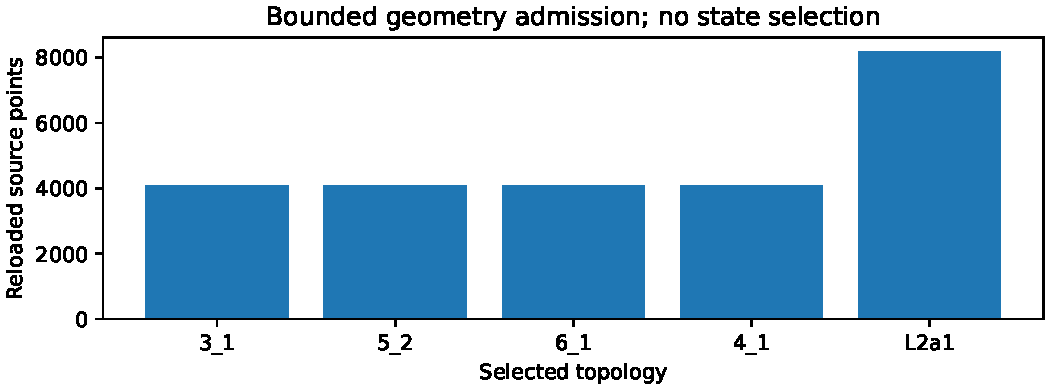
\includegraphics[width=0.85\linewidth]{figures/source_points.pdf}\caption{Actual source-native point counts reloaded in this admission smoke. Counts are not a convergence or physical-quality score.}\end{figure}
\subsection*{Unresolved scientific evidence}
Each BASIC topology has one selected provider. Independent provider convergence cannot close, including L2a1. No stationary endpoint, converged Hessian, ringdown or state-selected handoff was computed. Existing scientific thresholds remain unchanged.


\IfFileExists{AUTO_RESULTS.tex}{% AUTO-GENERATED. Do not edit.
\subsection*{Automatic run provenance}
\begin{longtable}{p{0.28\linewidth}p{0.64\linewidth}}
\toprule
Field & Recorded value \\
\midrule
Run ID & 20261026T222010309231Z-\allowbreak{}f16c0b6c \\
Run phase & BLIND \\
Protocol bundle SHA-256 (byte exact) & d788e4106e22\allowbreak{}f344c822c499\allowbreak{}8a4f7f574528\allowbreak{}2ecf5a0d06bb\allowbreak{}44cb464116e9\allowbreak{}645a \\
Portable protocol diagnostic SHA-256 & unavailable \\
Framework schema & SST-\allowbreak{}FALSIFIER-\allowbreak{}PROTOCOL-\allowbreak{}2 \\
Python & 3.14.3 (tags/\allowbreak{}v3.14.3:323c59a, Feb  3 2026, 16:04:56) [MSC v.1944 64 bit (AMD64)] \\
Platform & Windows-\allowbreak{}11-\allowbreak{}10.0.26300-\allowbreak{}SP0 \\
Science evidence SHA-256 & e975aadbbf54\allowbreak{}8ca81c0c2b91\allowbreak{}00a769d842e4\allowbreak{}34e29ec8aec7\allowbreak{}ae6bca8128aa\allowbreak{}8434 \\
Final output manifest & See OUTPUT\_\allowbreak{}MANIFEST.json (finalized after PDF and report metadata) \\
\bottomrule
\end{longtable}
\subsubsection*{Gate ledger}
\begingroup\small\setlength{\tabcolsep}{3pt}\begin{longtable}{p{0.07\linewidth}p{0.19\linewidth}p{0.31\linewidth}p{0.29\linewidth}}
\toprule
Gate & Status & Question & Reason \\
\midrule
{\ttfamily\scriptsize G0} & {\ttfamily\footnotesize PASS} & Is the frozen v0.6.0 protocol intact and runtime/\allowbreak{}implementation provenance self-\allowbreak{}consistent? & 112 qualified framework files and public scoped migration protocol verified; not a complete physical blind FREEZE. \\
{\ttfamily\scriptsize G1} & {\ttfamily\footnotesize PASS} & Is the run exactly bound to the E013 common-\allowbreak{}carrier manifest, with all E011 source geometries reloaded and hash-\allowbreak{}verified? & Fresh E013 selector binding; exact current E011 joins, raw hashes and parsed geometry hashes verified. \\
{\ttfamily\scriptsize G2} & {\ttfamily\footnotesize UNRESOLVED} & Do rigid-\allowbreak{}objectivity, constrained-\allowbreak{}objective identity, Armijo monotonicity and topology-\allowbreak{}proxy controls pass? & No scientific evaluator implemented for this gate; not executed \\
{\ttfamily\scriptsize G3} & {\ttfamily\footnotesize UNRESOLVED} & Can the fixed target-\allowbreak{}free constrained-\allowbreak{}objective selector drive the preregistered carrier fraction to stationary states, with numerical descent failures retained as UNRESOLVED? & No scientific evaluator implemented for this gate; not executed \\
{\ttfamily\scriptsize G4} & {\ttfamily\footnotesize UNRESOLVED} & Does the same frozen constrained-\allowbreak{}objective selector generalize without refit to registered confirmation topologies? & No scientific evaluator implemented for this gate; not executed \\
{\ttfamily\scriptsize G5} & {\ttfamily\footnotesize UNRESOLVED} & Does C++/\allowbreak{}OpenMP FP64 reproduce Python/\allowbreak{}NumPy FP64 for the state-\allowbreak{}selection energy kernel? & No scientific evaluator implemented for this gate; not executed \\
{\ttfamily\scriptsize G6} & {\ttfamily\footnotesize UNRESOLVED} & If available, does framework GPU/\allowbreak{}DD32 screening evidence remain consistent without being promoted to certification? & No scientific evaluator implemented for this gate; not executed \\
{\ttfamily\scriptsize G7} & {\ttfamily\footnotesize UNRESOLVED} & Do independently sourced provider anchors of the same topology converge to the same stationary endpoint without unresolved optimizer cases? & No scientific evaluator implemented for this gate; not executed \\
{\ttfamily\scriptsize G8} & {\ttfamily\footnotesize UNRESOLVED} & Are stationarity-\allowbreak{}qualified endpoints locally stable under a finite-\allowbreak{}difference-\allowbreak{}converged constrained Hessian and bounded ringdown on the same objective? & No scientific evaluator implemented for this gate; not executed \\
{\ttfamily\scriptsize G10} & {\ttfamily\footnotesize UNRESOLVED} & For source-\allowbreak{}energy-\allowbreak{}sensitive topologies, does numerically resolved state selection collapse provider spread toward a common endpoint? & No scientific evaluator implemented for this gate; not executed \\
{\ttfamily\scriptsize G11} & {\ttfamily\footnotesize UNRESOLVED} & Are clearance and link-\allowbreak{}drift topology proxies preserved along every completed state-\allowbreak{}selection path? & No scientific evaluator implemented for this gate; not executed \\
{\ttfamily\scriptsize G12} & {\ttfamily\footnotesize UNRESOLVED} & Can at least one provider-\allowbreak{}converged stationary, Hessian-\allowbreak{}converged, stable state be frozen as an A057-\allowbreak{}compatible handoff? & No scientific evaluator implemented for this gate; not executed \\
{\ttfamily\scriptsize G22} & {\ttfamily\footnotesize UNRESOLVED} & What is the overall state-\allowbreak{}selection evidence classification when numerical unresolved states are kept distinct from scientific FAIL? & No scientific evaluator implemented for this gate; not executed \\
{\ttfamily\scriptsize G9} & {\ttfamily\footnotesize DEFERRED} & After a completed FULL/\allowbreak{}CERTIFY blind run, do reveal and commitment checks verify exactly? & Reveal is outside the authorized admission-\allowbreak{}smoke scope. \\
\bottomrule
\end{longtable}\endgroup
\subsubsection*{Scientific qualification (separate from measured gate outcomes)}
\begingroup\small\setlength{\tabcolsep}{3pt}\begin{longtable}{p{0.13\linewidth}p{0.37\linewidth}p{0.38\linewidth}}
\toprule
Gate & Evidence qualification & Blocking prerequisites \\
\midrule
G0 & QUALIFIED & none \\
G1 & QUALIFIED & none \\
G2 & UNRESOLVED & none \\
G3 & UNRESOLVED & none \\
G4 & UNRESOLVED & none \\
G5 & UNRESOLVED & none \\
G6 & UNRESOLVED & none \\
G7 & UNRESOLVED & none \\
G8 & UNRESOLVED & none \\
G10 & UNRESOLVED & none \\
G11 & UNRESOLVED & none \\
G12 & UNRESOLVED & none \\
G22 & UNRESOLVED & none \\
G9 & DEFERRED & none \\
\bottomrule
\end{longtable}\endgroup
\subsubsection*{Backend manifest}
\begingroup\footnotesize\begin{verbatim}
{
  "actual_backend": "Python/NumPy FP64 source parsing",
  "authority": "SOURCE_ADMISSION_ONLY",
  "gpu_used": false,
  "native_executed": false,
  "physical_qualification": "NOT_RUN",
  "schema": "SST-BACKEND-MANIFEST-2"
}
\end{verbatim}\endgroup
\subsubsection*{Source manifest}
\begingroup\footnotesize\begin{verbatim}
{
  "manifest_sha256": 
"d5e9f6cced7be46c0b7038fbfa0d42f3511d0939dc1bcc7d156373d859eaac6e",
  "schema": "SST-SOURCE-MANIFEST-2",
  "sources": [
    {
      "catalog_id": "E011",
      "evidence_class": "simulation",
      "exists": false,
      "independence_family": "gilbert",
      "path": null,
      "provenance_family": null,
      "registry_hint": {
        "catalog_id": "E011",
        "hits": []
      },
      "role": "Admitted geometry; static authority only",
      "source_id": "CAR_f0023c079d7502c1",
      "version": "v0.3.0"
    },
    {
      "catalog_id": "E011",
      "evidence_class": "simulation",
      "exists": false,
      "independence_family": "gilbert",
      "path": null,
      "provenance_family": null,
      "registry_hint": {
        "catalog_id": "E011",
        "hits": []
      },
      "role": "Admitted geometry; static authority only",
      "source_id": "CAR_97c30a73f3ab9b85",
      "version": "v0.3.0"
    },
    {
      "catalog_id": "E011",
      "evidence_class": "simulation",
      "exists": false,
      "independence_family": "gilbert",
      "path": null,
      "provenance_family": null,
      "registry_hint": {
        "catalog_id": "E011",
        "hits": []
      },
      "role": "Admitted geometry; static authority only",
      "source_id": "CAR_154a6dad7b515c61",
      "version": "v0.3.0"
    },
    {
      "catalog_id": "E011",
      "evidence_class": "simulation",
      "exists": false,
      "independence_family": "gilbert",
      "path": null,
      "provenance_family": null,
      "registry_hint": {
        "catalog_id": "E011",
        "hits": []
      },
      "role": "Admitted geometry; static authority only",
      "source_id": "CAR_fc293690c619f8ca",
      "version": "v0.3.0"
    },
    {
      "catalog_id": "E011",
      "evidence_class": "simulation",
      "exists": false,
      "independence_family": "gilbert",
      "path": null,
      "provenance_family": null,
      "registry_hint": {
        "catalog_id": "E011",
        "hits": []
      },
      "role": "Admitted geometry; static authority only",
      "source_id": "CAR_a3ffb7da038a2929",
      "version": "v0.3.0"
    }
  ],
  "workbench_root": "C:\\workspace\\projects\\SST-Workbench"
}
\end{verbatim}\endgroup
}{No run results are embedded in the source release.}
% SST-REPORT-SECTION:INTERPRETATION
\section{Interpretation}
A stationary point is not a stable state merely because $\nabla U_c\simeq0$. Provider convergence and positive local stability are independent requirements. Numerical inability to establish descent or Hessian-sign convergence remains unresolved. Only topologies satisfying provider convergence, stationarity, converged nonnegative local stability and bounded ringdown are eligible for the state-selected handoff.
% SST-REPORT-SECTION:REPRODUCIBILITY
\section{Reproducibility}
From this version directory run \texttt{run\_all.cmd SELFTEST} or \texttt{run\_all.cmd ADMISSION\_SMOKE}. CPython 3.14, NumPy, matplotlib, pytest and pdflatex are required, together with this Workbench's exact pinned framework, E010 parser and E011 sources. FULL, CERTIFY and REVEAL are blocked. The successor is disabled for global E013 discovery to preserve the enabled historical member without duplicates. Per-run parent PDFs and ZIPs are immutable; earlier output trees retain their run IDs.
\begin{thebibliography}{99}
\bibitem{Moffatt1969} H.~K. Moffatt, ``The degree of knottedness of tangled vortex lines,'' \emph{J. Fluid Mech.} 35, 117--129 (1969). DOI: \href{https://doi.org/10.1017/S0022112069000991}{10.1017/S0022112069000991}.
\bibitem{Saffman1992} P.~G. Saffman, \emph{Vortex Dynamics}. Cambridge University Press (1992). DOI: \href{https://doi.org/10.1017/CBO9780511624063}{10.1017/CBO9780511624063}.
\bibitem{Bishop1975} R.~L. Bishop, ``There is More than One Way to Frame a Curve,'' \emph{Amer. Math. Monthly} 82, 246--251 (1975). DOI: \href{https://doi.org/10.1080/00029890.1975.11993807}{10.1080/00029890.1975.11993807}.
\end{thebibliography}
\end{document}
